
\definecolor{cffffff}{RGB}{255,255,255}


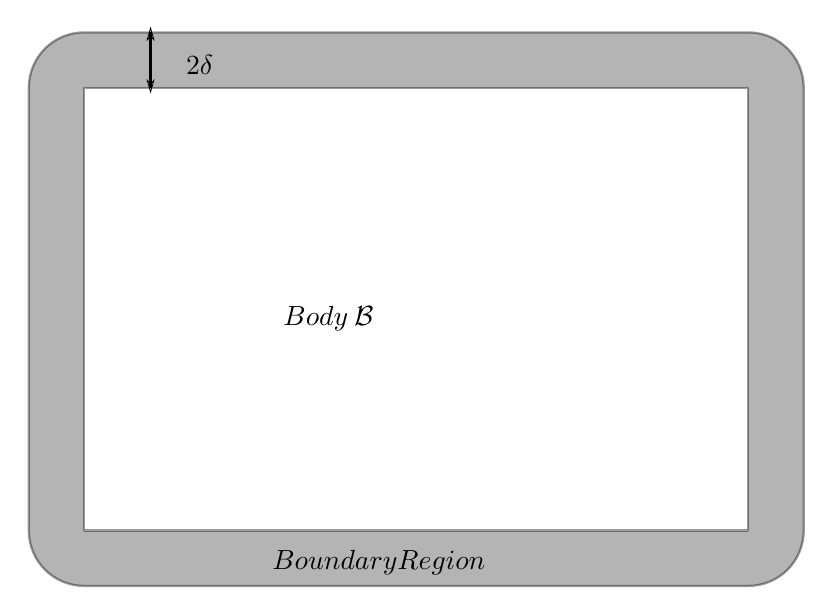
\begin{tikzpicture}[y=0.80pt, x=0.8pt,yscale=-1, inner sep=0pt, outer sep=0pt]
\begin{scope}[shift={(0,-652.36218)}]
  \path[shift={(0,652.36218)},draw=black,fill=black,line join=round,miter
    limit=4.00,draw opacity=0.392,fill opacity=0.294,nonzero rule,line
    width=0.823pt] (50.0000,25.0000) -- (350.0000,25.0000) .. controls
    (363.8500,25.0000) and (375.0000,36.1500) .. (375.0000,50.0000) --
    (375.0000,250.0000) .. controls (375.0000,263.8500) and (363.8500,275.0000) ..
    (350.0000,275.0000) -- (50.0000,275.0000) .. controls (36.1500,275.0000) and
    (25.0000,263.8500) .. (25.0000,250.0000) -- (25.0000,50.0000) .. controls
    (25.0000,36.1500) and (36.1500,25.0000) .. (50.0000,25.0000) -- cycle;
  \path[shift={(0,652.36218)},draw=black,fill=cffffff,line join=round,miter
    limit=4.00,draw opacity=0.392,nonzero rule,line width=0.823pt,rounded
    corners=0.0000cm] (50.0000,50.0000) rectangle (350.0000,250.0000);
    \path[color=black,fill=black,line width=1.200pt] (79.2500,677.3622) --
      (79.2500,702.3622) -- (80.7500,702.3622) -- (80.7500,677.3622) --
      (79.2500,677.3622) -- cycle;
    \path[draw=black,even odd rule,line width=0.300pt] (80.0000,679.1622) --
      (81.5000,680.6622) -- (80.0000,675.4122) -- (78.5000,680.6622) --
      (80.0000,679.1622) -- cycle;
    \path[draw=black,even odd rule,line width=0.300pt] (80.0000,700.5622) --
      (78.5000,699.0622) -- (80.0000,704.3122) -- (81.5000,699.0622) --
      (80.0000,700.5622) -- cycle;
  \path[shift={(0,652.36218)},fill=black] (96.071426,43.92857) node[above right]
    (text4653) {$2\delta$};
  \path[fill=black] (140,812.36218) node[above right] (text4657) {$\text{Body}\:
    \mathcal{B}$};
  \path[fill=black] (135,922.36218) node[above right] (text4661) {$\text{Boundary
    Region}$};
\end{scope}

\end{tikzpicture}

